\documentclass[12pt, letter]{article}

\usepackage[rounded]{syntax}
\usepackage{tikz}
\usetikzlibrary{
	arrows.meta,
}
\title{Lab 2}
\author{James You}

\begin{document}
	\maketitle
	\newpage
	\section*{Lab Question 1}
		\texttt{HexIntegerLiteral:}
		\begin{syntdiag}
			<HexNumeral> 
			\begin{stack} \\
				<IntegerTypeSuffix> 
			\end{stack}
		\end{syntdiag}
		\texttt{IntegerTypeSuffix:}
		\begin{syntdiag}
			\begin{stack}
				l \\
				L 
			\end{stack}
		\end{syntdiag}
		\texttt{HexNumeral:}
		\begin{syntdiag}
			\begin{stack}
			0x <HexDigits> \\
			0X <HexDigits>
			\end{stack}
		\end{syntdiag}
		\texttt{HexDigits:}
		\begin{syntdiag}
			\begin{rep} 
				<HexDigit> \\
				\begin{stack}
					<HexDigitsandUnderscores>
				\end{stack}
			\end{rep}
		\end{syntdiag}
		\texttt{HexDigit:}
		\begin{syntdiag}
			\begin{stack}
			0 .. 9 \\
			a .. f \\
			A .. F 
			\end{stack}
		\end{syntdiag}
		\texttt{HexDigitsandUnderscores:}
		\begin{syntdiag}
			<HexDigitorUnderscore>
			\begin{rep} \\
				\begin{stack} 
					<HexDigitorUnderscore>
				\end{stack}
			\end{rep}
		\end{syntdiag}
		\texttt{HexDigitorUnderscore:}
		\begin{syntdiag}
			\begin{stack}
				<HexDigit> \\
				\_
			\end{stack}
		\end{syntdiag}
	\newpage
	\section*{Lab Question 2}
	\paragraph*{a)}
	The set of all sentences over $\{a, b\}$ including the empty string $\epsilon$.
	\paragraph*{b)}
	The set of all sentences over $\{a, b\}$ including $\epsilon$ such that the strings must have an even number of occurrences of $b$, otherwise, there must be no occurrences of $b$.
	\paragraph*{c}
	The set of all sentences over $\{a, b, c\}$ including $\epsilon$ such that $b$ occurs the same amount of times as $c$ and the string must end in either $a$ or $c$.
	\section*{Lab Question 3}
	\paragraph*{a)}
	Let $r_1 = bd\ |\ bc^*d$ and $r_2 = bc^*d$, the following expressions are equivalent. To prove this, we can first observe $L(r_2) \subset L(r_1)$ because all patterns which exist in $r_2$ exist in $r_1$, therefore any language generated through $r_2$ can be generated by $r_1$. Secondly, If $r_2$ is a subset of $r_1$, we then must prove that the sentence $bd$ can be generated by $r_2$. We can assert the language generated by $r_2$ to be of the form $\{bc^nd\ |\ n \geq 0\}$, the base case of $n = 0$ satisfies $bc^0d = bd$. Therefore $L(r_2) \subseteq L(r_1)$ and $L(r_1) \subseteq L(r_2)$. Therefore the regular expressions are equivalent because they generate the same language and are subsets of each other.
	
	\paragraph{b)} 
	Let $r_1 = ab\ |\ bd^*$ and $r_2 = [a]bd^*$. The two grammars are not equivalent. This can be proved through a simple counterexample of the sentence $s = abd$. $r_1$ cannot match $s$ while $r_2$ can.
	
	\paragraph{c)}
	Let $r_1 = (a\ |\ ba)^*$ and $r_2 = (a\ |\ b)^*$. We can see from observation that $L(r_2)$ is the set of all strings over $\{a, b\}$. Then it is clear that $L(r_1) \subset L(r_2)$. However $L(r_2) \subseteq L(r_1)$ is not true. We can prove this through the use of counterexample of $s = abb$. The sentence $s$ can only be matched by $r_2$. Therefore the regular expressions are not equivalent.
	
	\section*{Lab Question 4}
	$r = a^*b(b\ \vert\ c)^*$
	\section*{Lab Question 5}
	\begin{grammar}
	<S> ::= <A> | <B> | <C>
	
	<A> ::= a<A> | $\epsilon$
	
	<B> ::= b<B> | $\epsilon$
	
	<C> ::= a<D> | $\epsilon$
	
	<D> ::= b<C>
	\end{grammar}

	\section*{Lab Question 6}
	
	
	
	\begin{tabular}{ l l l l }
		Step & Q' & R' & \\
		0 & \{0\} & $\emptyset$ & \\  
		1 & \{0\} & $\emptyset$ & $\delta(0, a) = \{0, 1\},\ \delta(0, b) = \{0\}$ \\
		2 & \{0, \{0, 1\}\} & \{\{0\} a $\rightarrow$ \{0, 1\}, \{\{0\} b $\rightarrow$ \{0\}\} &\ \\
		3 & \{0, \{0, 1\}\} & '' & $\delta(\{0, 1\}, a) = \{0, 1\},\ \delta(\{0, 1\}, b) = \{0, 1\}$ \\
	\end{tabular}

	\begin{center}
		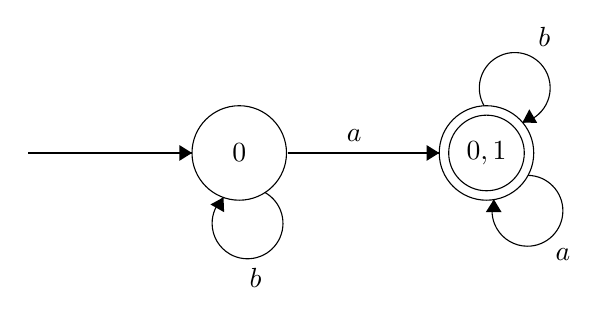
\begin{tikzpicture}[scale=0.2]
		\tikzstyle{every node}+=[inner sep=0pt]
		\draw [black] (20.2,-30.1) circle (3);
		\draw (20.2,-30.1) node {$0$};
		\draw [black] (35.9,-30.1) circle (3);
		\draw (35.9,-30.1) node {$0,1$};
		\draw [black] (35.9,-30.1) circle (2.4);
		\draw [black] (21.827,-32.607) arc (60.70984:-227.29016:2.25);
		\draw (21.24,-37.39) node [below] {$b$};
		\fill [black] (19.2,-32.92) -- (18.37,-33.37) -- (19.24,-33.86);
		\draw [black] (6.8,-30.1) -- (17.2,-30.1);
		\fill [black] (17.2,-30.1) -- (16.4,-29.6) -- (16.4,-30.6);
		\draw [black] (23.3,-30.1) -- (32.9,-30.1);
		\draw (28,-29) node [left] {$a$};
		\fill [black] (32.9,-30.1) -- (32.1,-29.6) -- (32.1,-30.6);
		\draw [black] (35.756,-27.115) arc (210.50143:-77.49857:2.25);
		\draw (39.57,-23.4) node [above] {$b$};
		\fill [black] (38.18,-28.17) -- (39.12,-28.19) -- (38.62,-27.33);
		\draw [black] (38.528,-31.522) arc (89.31121:-198.68879:2.25);
		\draw (40.75,-36.11) node [below] {$a$};
		\fill [black] (36.37,-33.05) -- (35.86,-33.85) -- (36.86,-33.86);
		\end{tikzpicture}
	\end{center}
	
	
\end{document}